\subsection{Modellierung eines vergleichbaren klassischen Fließfertigungsprozesses}
\label{Modellierung}

Nach Erarbeitung der Möglichkeiten von selbststeuernden Prozessen anhand des
Fallbeispiels, wird nun ein klassischer Fließfertigungsprozess modelliert.
Dieser soll mit dem selbststeuernden Prozess verglichen werden, um Möglichkeiten
und Grenzen von selbststeuernden Prozessen zu identifizieren. Hierzu ist es
notwendig den Fließfertigungsprozess so zu modellieren, dass ebenfalls
PKW-Rücklicher produziert werden, damit eine gleiche Basis für den Vergleich
beider Prozesse besteht. Der Aufbau der klassischen Fließfertigung stellt sich
dabei folgendermaßen dar:

\begin{figure}[htb] 
\centering
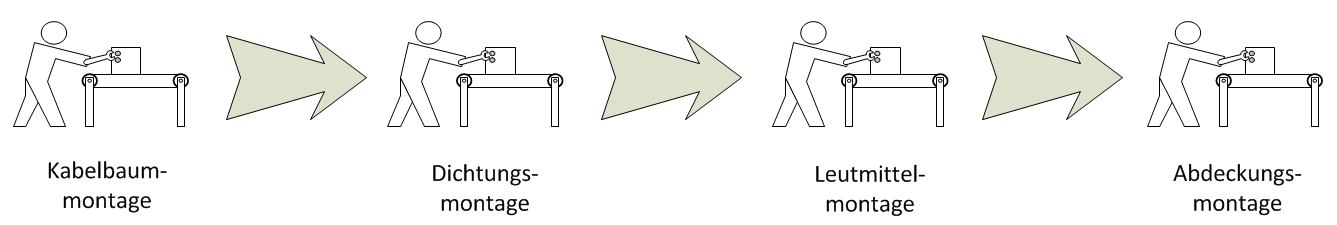
\includegraphics[width=1.0\textwidth]{fliessfertigung_4.png}
\caption[Montagestation]{Darstellung der PKW-Rücklichterproduktion als Fließfertigung\protect\footnotemark}
\label{fig:Fliessfertigung}
\end{figure}
\footnotetext{eigene Darstellung}
%TODO \caption was hat das zusagen []?

Die vorangegangene Skizze stellt dar, dass der in unserem Sinne klassische
Fertigungsprozess eine Fließfertigung ohne Abzweigungen ergibt. Der
Montageprozess läuft dabei so ab, dass das Reflektor-Gussteil über ein Fließband
einzelne Fertigungsstationen in einer fest vorgegebenen Reihenfolge durchläuft.
So wird bei der ersten Station der Kabelbaum für die PKW-Rücklichter montiert
und bei der zweiten Station die Dichtung angebracht. Um verschiedene Varianten
von Rücklichtern herstellen zu können, wird keine Verzweigung zu den einzelnen
Fertigungsvarianten genutzt, sondern es werden an der nächsten Station nur die
der Variante entsprechenden Bauteile montiert.

Die Wahl der Bauteile erfolgt dabei anhand eines vorher definierten
Produktionsplanes.\footnote{\citet[S.~331]{arnold2008}} So werden bei der
dritten Fertigungsstation die Leuchtmittel und bei der Vierten die Blenden montiert. Je nach geforderter Variante im
Produktionsplan, werden dementsprechend die zusammengehörigen Leuchtmittel und
Blenden nacheinander verbaut. Hierbei ist aber zu beachten, dass je nach
gewünschter Variante des Rücklichtes die Fertigungsstation dementsprechend
umgerüstet werden muss, wodurch Rüstzeiten beim Wechsel der Variante entstehen
können. Den letzten Schritt des Montageprozesses stellt der Einbau der Blende
dar. Nach diesem Schritt ist der Montageprozess für das PKW-Rücklicht
abgeschlossen.
 